\documentclass[11pt]{report}
\usepackage{StyleSheets/main}
\begin{document}

\chapter{Conceptual Design}\label{ch:conceptual-design}

\section*{Design Strategy}
Before the initial design process had begun, it was clear to the team that there would be a trade-off between complexity and efficiency --- as such, it was determined that the complexity of the system would have to increase greatly in order to get the maximum potential performance from the robot. The following designs are variations of the previous, with each design increasing in complexity.
\par Other teams reduced the amount of electrical components that connected to the Teensy 4.1 microcontroller to reduce the complexity of the code base, seen in \cref{ap:code}. This did not influence the design of this robot as the code base was designed from the ground up to be a modular system, utilizing an object oriented approach in \cplusplus{}, ensuring no extra code needed to be written or maintained the more sensors were added to the cart. Consequently, the design process was unrestricted by the quantity or variety of sensors available, permitting a more flexible approach to design.

\subsection*{Abbreviations used in Drawings}
\begin{itemize}
    \item \gls{US}
    \item \gls{CS}
    \item \gls{IRS}
    \item \gls{omni}
    \item \gls{FS}
    \item \gls{B}
\end{itemize}

\newpage
\section{Design 1}\label{sec:design1}
\begin{figure}[H]
    \centering
    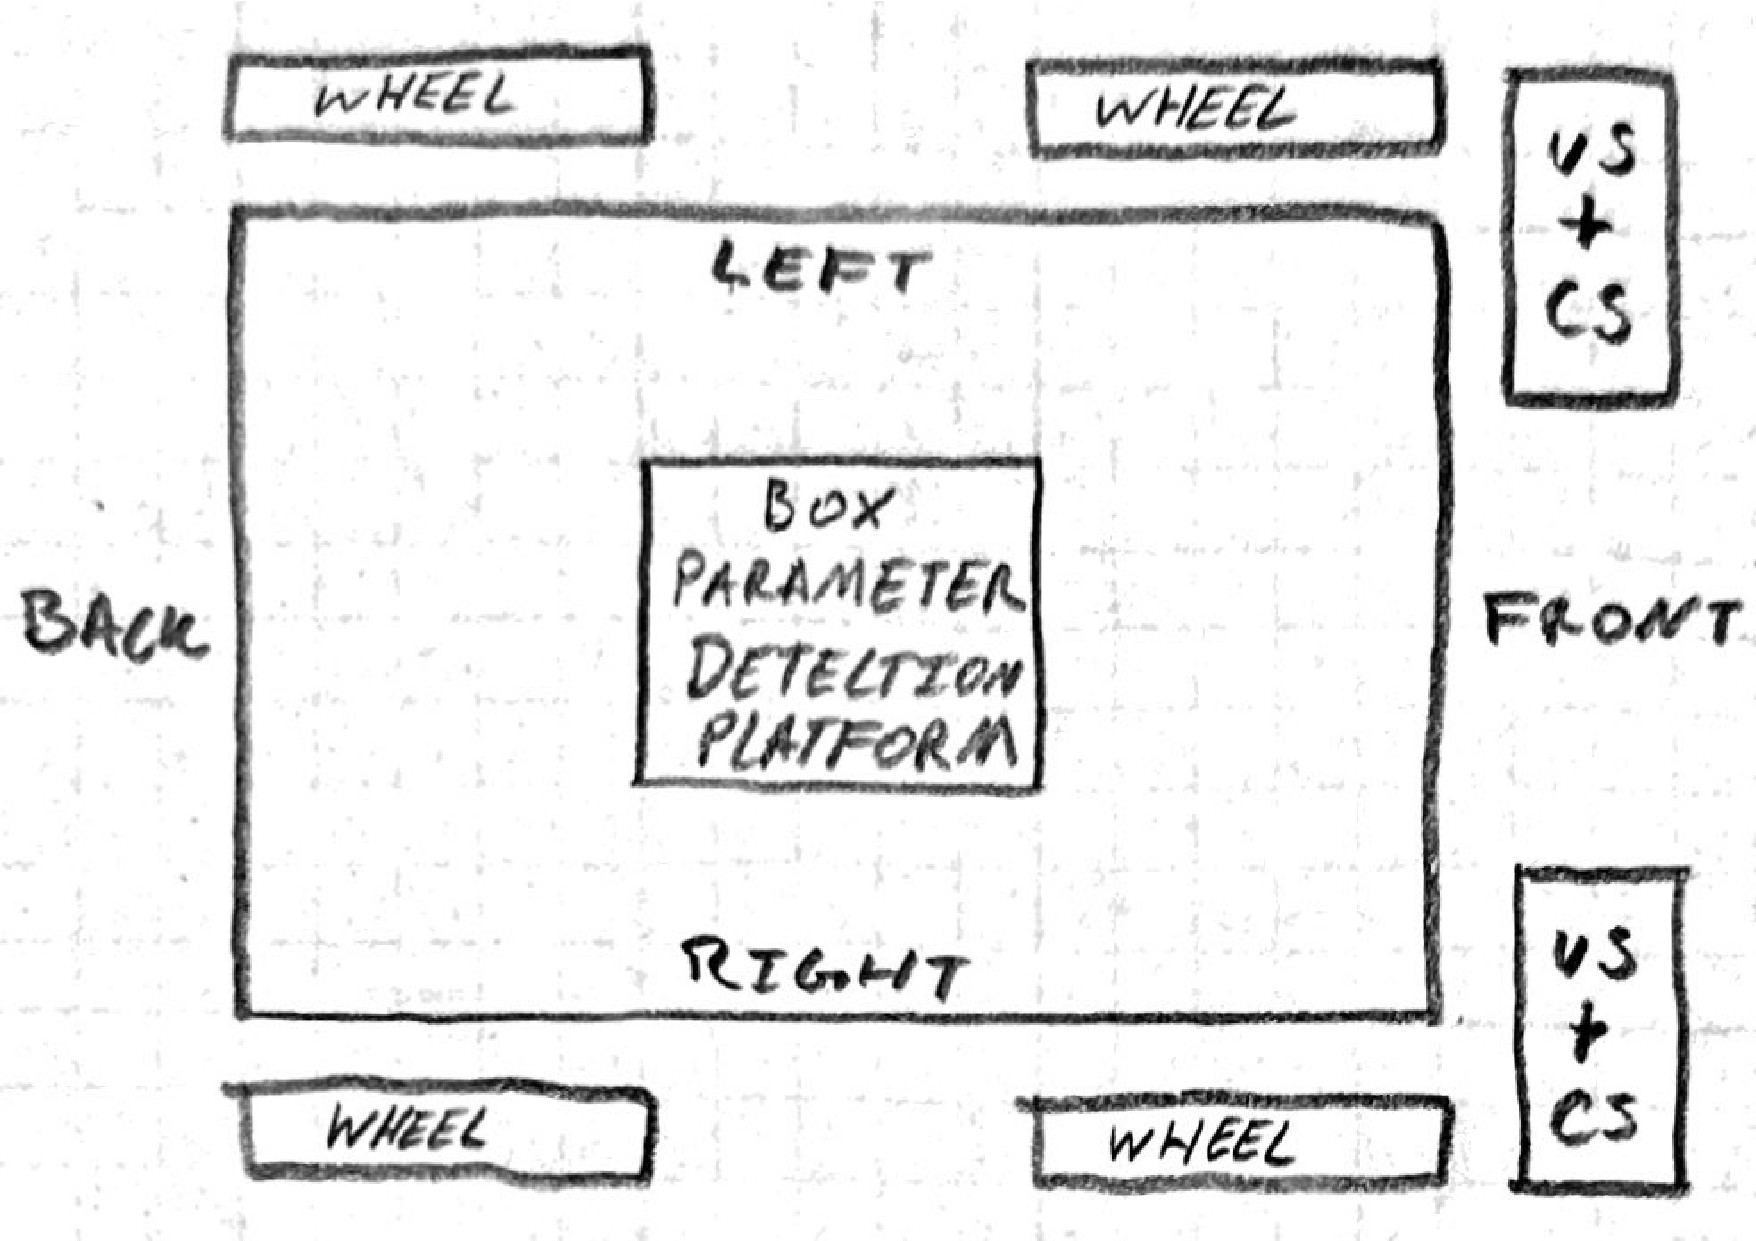
\includegraphics[width=0.5\linewidth]{Images//Designs/Design1a.pdf}
    \caption{Design 1a --- simplified layout of movement and sensor systems}
    \label{fig:design1a}
\end{figure}
The first design is an adaptation of the fundamental designs demonstrated throughout the prerequisite course, Integration I, for the sake of setting a baseline. Efficiency and speed are sacrificed for simple movement and sensor algorithms.

\begin{description}
    \item[Wheel Configuration --] This design utilizes a standard 2x2 wheel configuration featuring standard 1 \gls{DoF} wheels. This configuration performed consistently, yet was problematic when it came to creating highly dynamic movement algorithms.
    %
    \item[Sensor Configuration --] The front corners are fitted with dual-purpose sensor mounts, containing both an \gls{RGB} color sensor and an ultrasonic sensor to be used for all spatial objectives: line following, boundary/obstacle/object detection, and directional orientation.
\end{description}

\begin{figure}[H]
    \centering
    \hspace*{6em}
    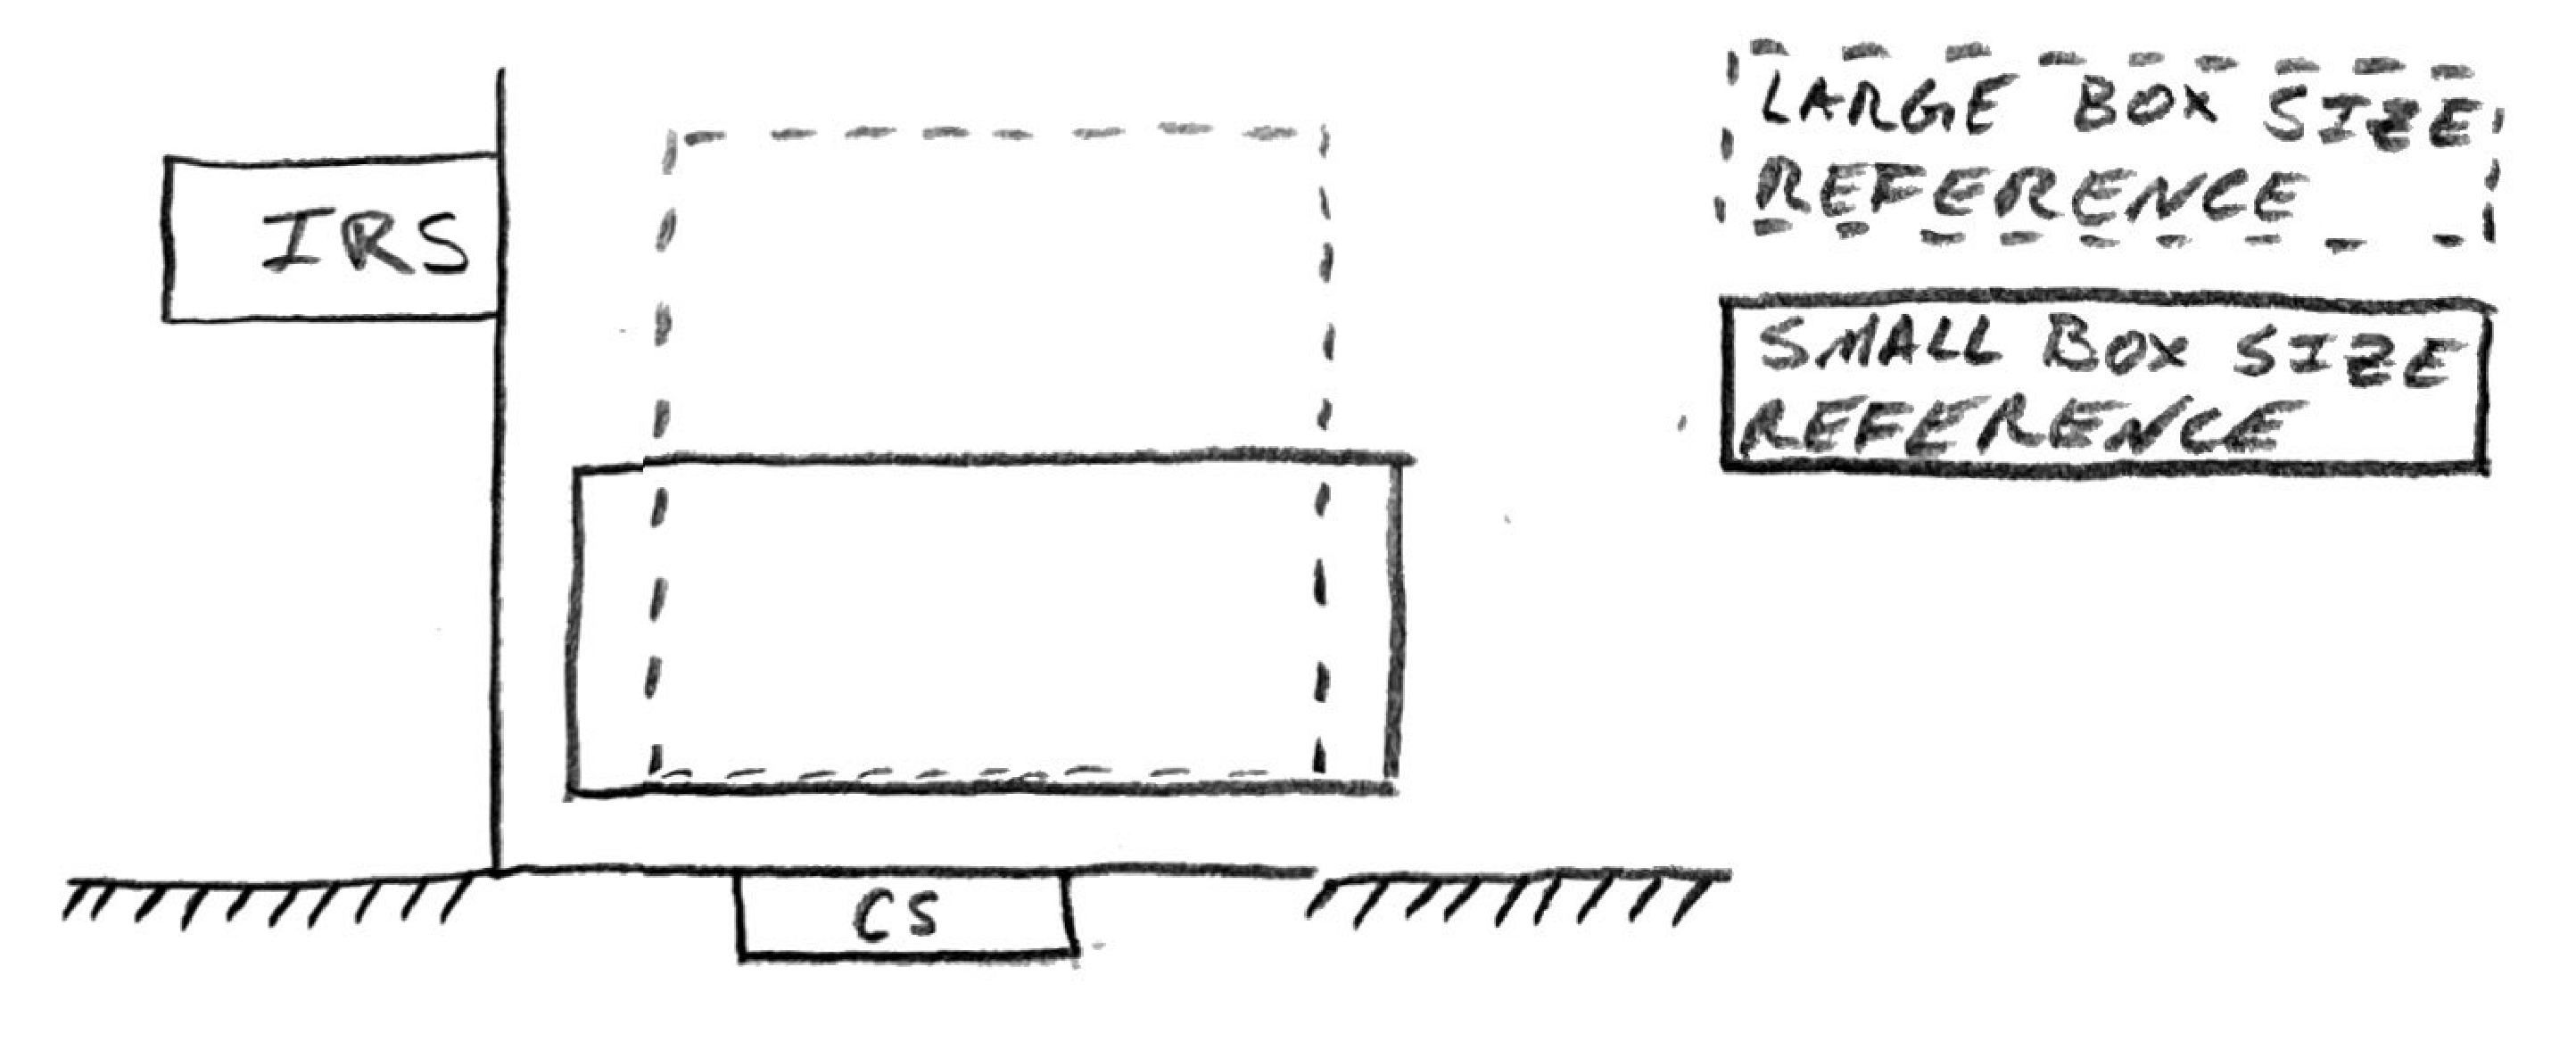
\includegraphics[width=0.6\linewidth]{Images//Designs/Design1b.pdf}
    \caption{Design 1b --- Box property detection platform with IRS}
    \label{fig:design1b}
\end{figure}
\begin{description}
    \item[Box Property Detection --]A gripper mechanism is to place the box onto a small platform on top of the robot that will contain an \gls{RGB} sensor to determine the package color, alongside an infrared sensor placed high enough to only detect the larger of two possible box sizes.
\end{description}

\newpage
\section{Design 2}\label{sec:design2}
\begin{figure}[H]
    \centering
    \hspace*{2em}
    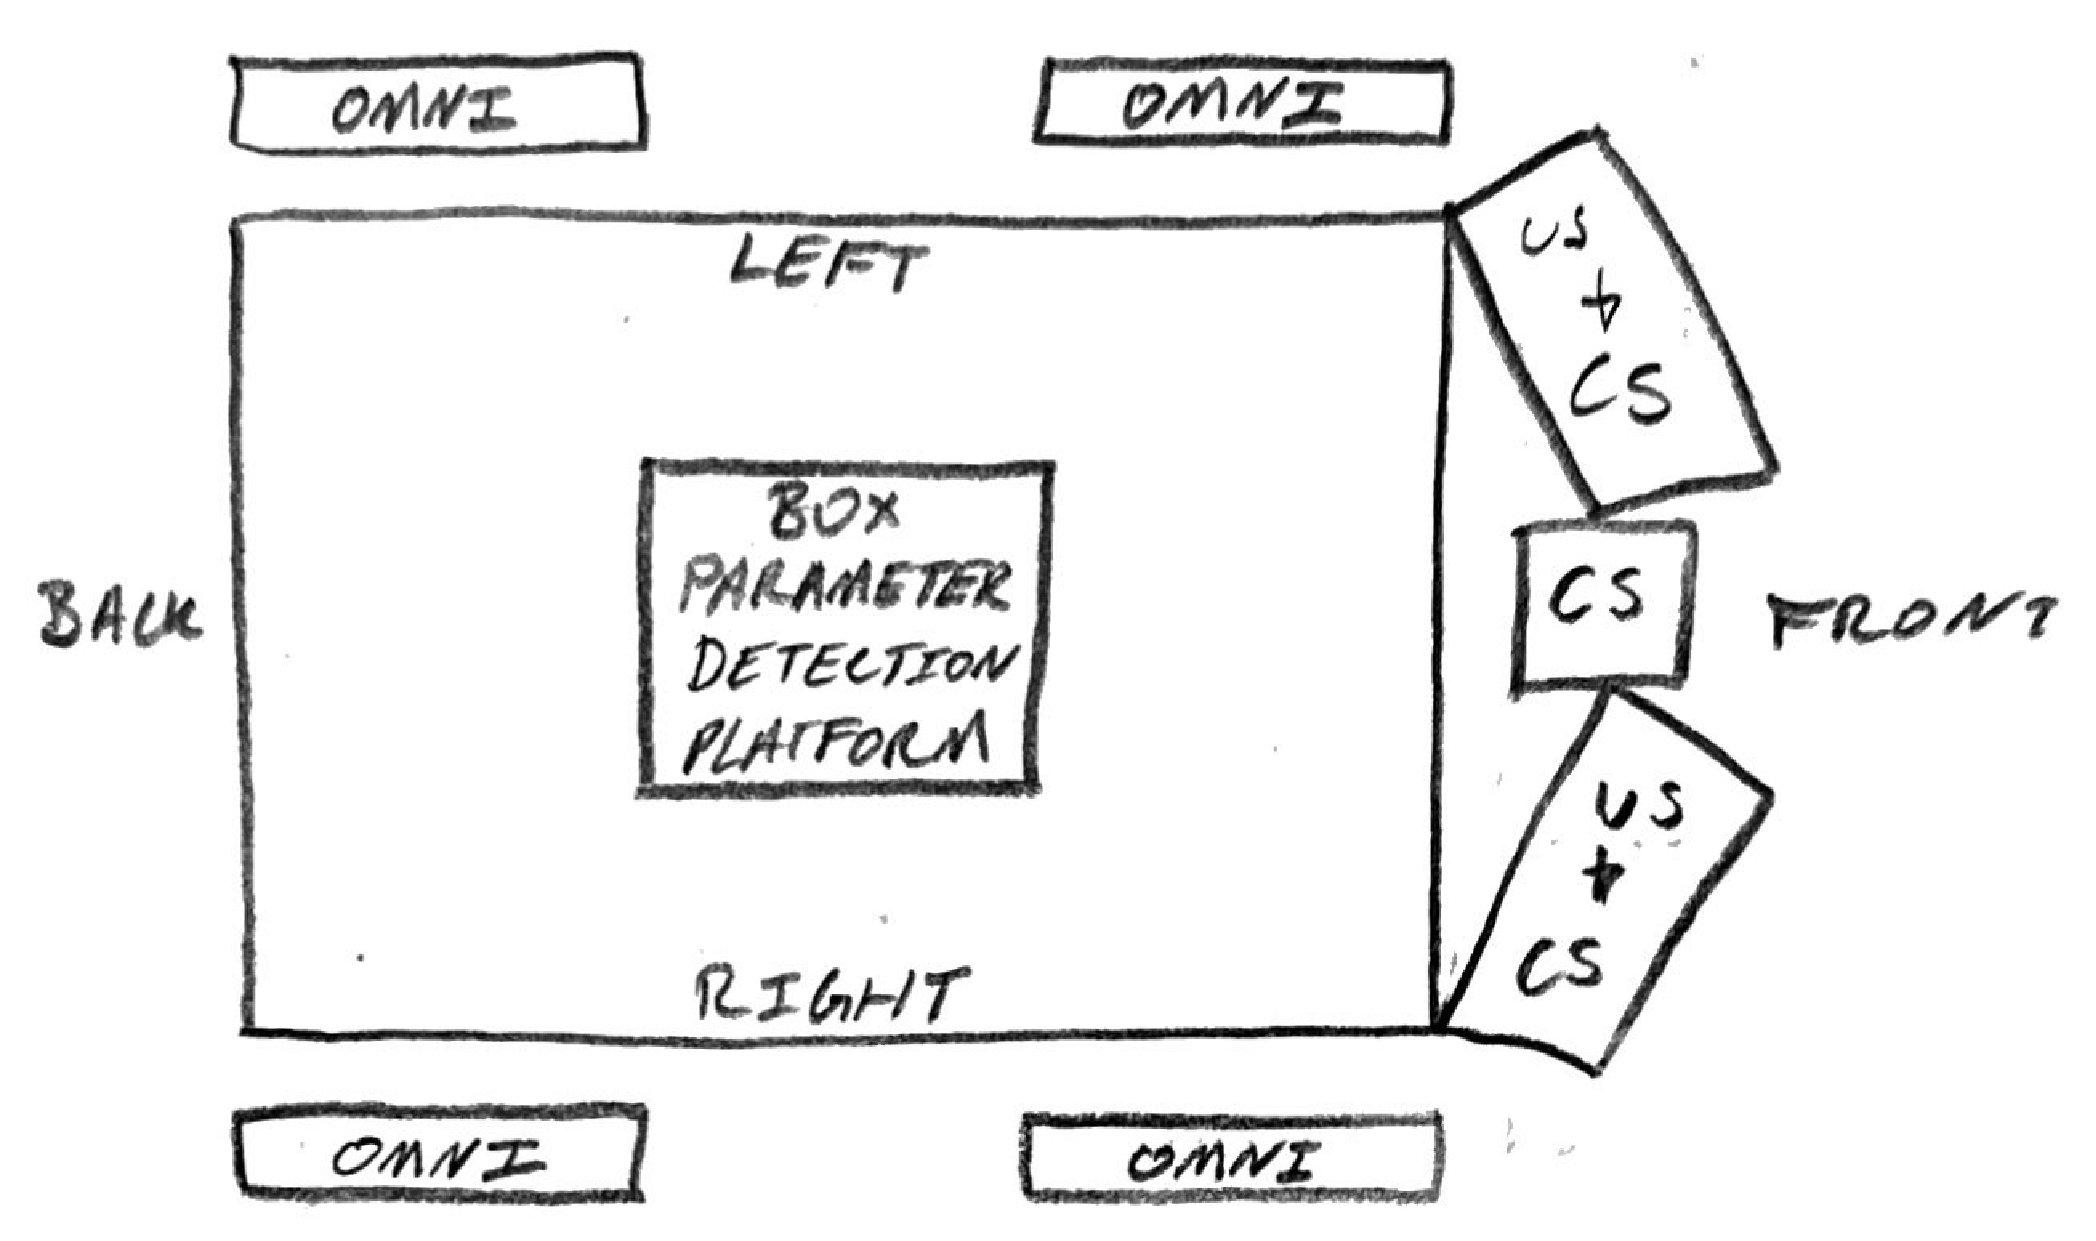
\includegraphics[width=0.5\linewidth]{Images//Designs/Design2a.pdf}
    \caption{Design 2a --- simplified layout of movement and sensor systems}
    \label{fig:design2a}
\end{figure}
The second design functions nearly identically to \cref{sec:design1} but with minor alterations to the sensor layout, as well as the introduction of \gls{omni}-wheels.

\begin{description}
    \item[Wheel Configuration --] This design still utilizes a standard 2x2 wheel configuration, but instead utilizes \gls{omni}-wheels with 2 \gls{DoF}. The implementation of \glspl{omni} fixes some of the aforementioned problems with dynamicism by enabling the robot to pivot more easily and with more control.
    %
    \item[Sensor Configuration --] This iteration uses a similar sensor layout to the previous, but this time the ultrasonic sensors are angled outward slightly, in theory, reducing the time it takes to identify objectives, subsequently increasing the overall efficiency of the system. Additionally, a third color sensor is attached to the center of the robot to increase the available information during line following functions.
\end{description}

\begin{figure}[H]
    \centering
    \hspace*{6em}
    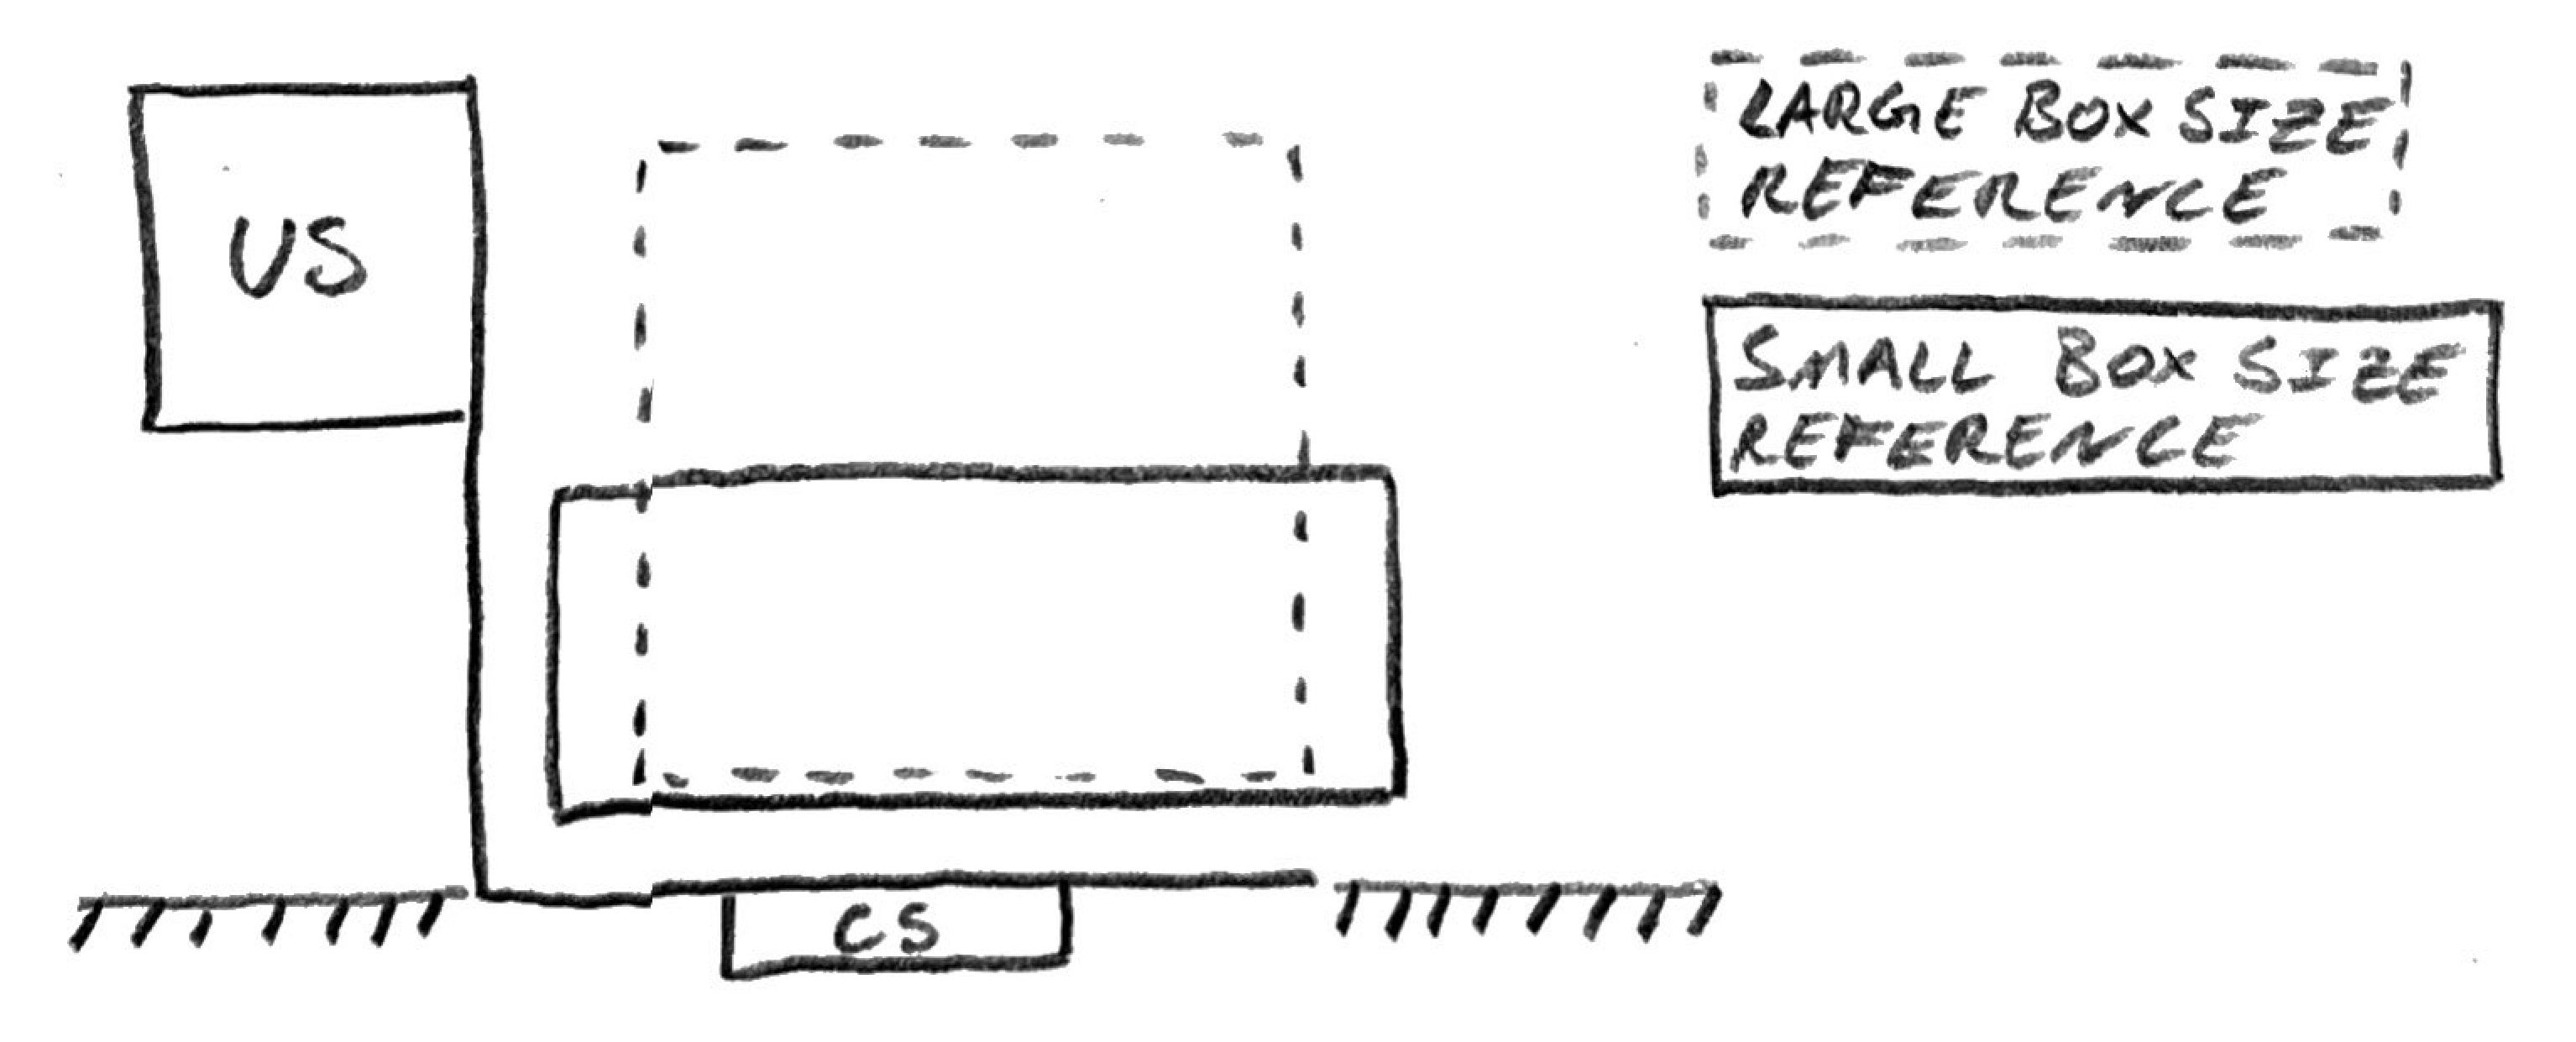
\includegraphics[width=0.6\linewidth]{Images//Designs/Design2b.pdf}
    \caption{Design 2b --- Box property detection platform with IRS}
    \label{fig:design2b}
\end{figure}
\begin{description}
    \item[Box Property Detection --]Again, a gripper mechanism places the box onto a platform that will then determine the properties of the package. An \gls{RGB} sensor is still used to get the color of the box, but an ultrasonic sensor replaces the \gls{IR} sensor. It should be noted that the swap from \gls{IRS} to \gls{US} was simply to provide another option during testing and assembly; there is no immediately identifiable benefit to using one over the other.
\end{description}

\newpage
\section{Design 3}\label{sec:design3}
\begin{figure}[H]
    \centering
    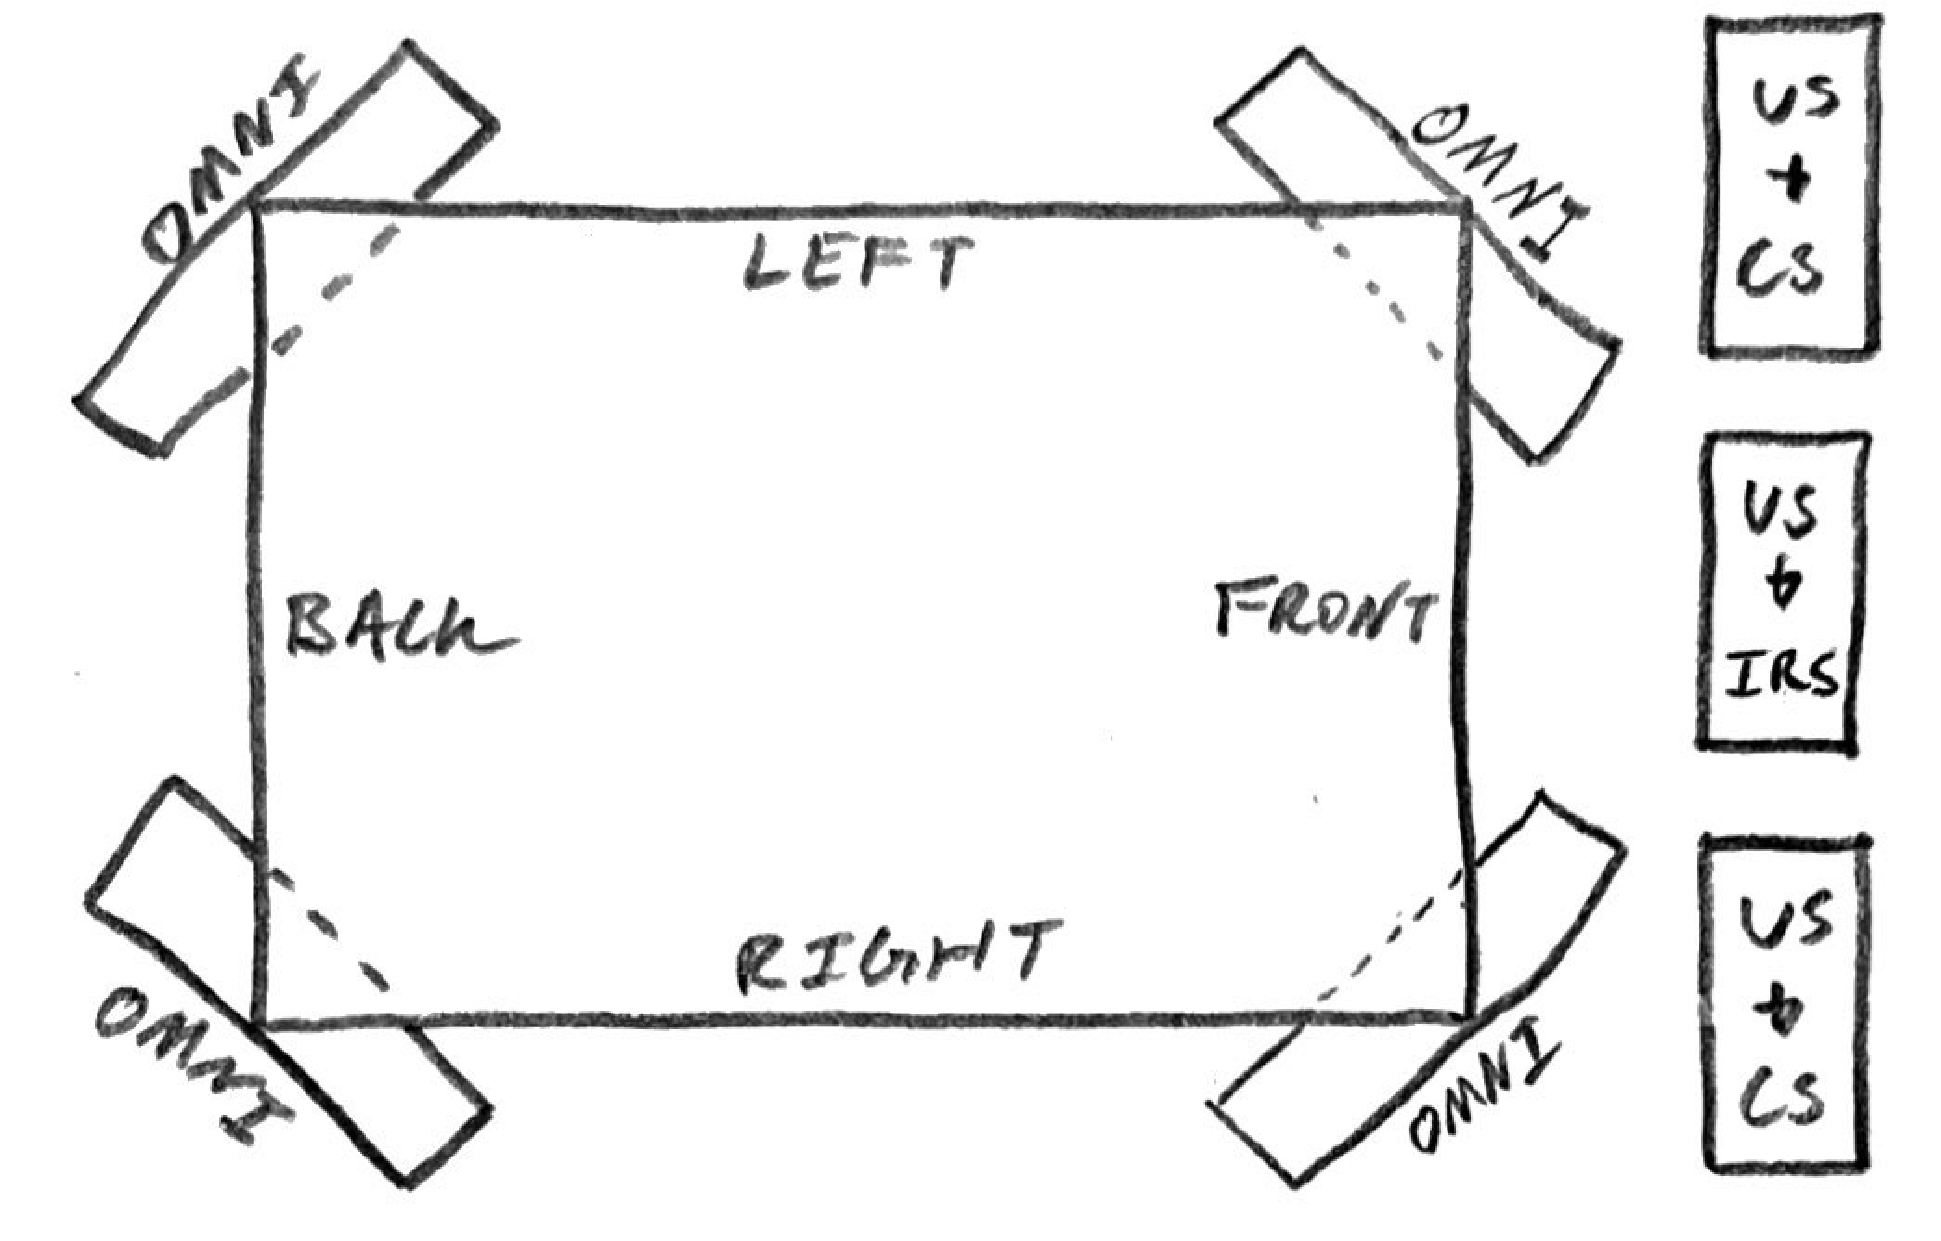
\includegraphics[width=0.5\linewidth]{Images//Designs/Design3a.pdf}
    \caption{Design 3a --- simplified layout of movement and sensor systems}
    \label{fig:design3a}
\end{figure}
The third design introduces a new movement strategy, and features a new sensor layout intended for smarter movement capabilities.
\begin{description}
    \item[Wheel Configuration --]The \glspl{omni} are now placed in a cornered configuration to enable crab-walking: linear translation in cardinal directions, or otherwise, via relative \gls{PWM} control.
    \item[Sensor Configuration --]The ultrasonic sensors on the sides have been reverted to the original forward-facing orientation due to the addition of a third ultrasonic sensor. The side ultrasonic sensors are intended to be in-line with the wheels to predict possible collisions across the whole robot, and the centrally located one allows for faster targeting of the pick-up-and-place platforms. Lastly, two or more centered \gls{IR} sensors are utilized for line-following purposes.
\end{description}
\begin{figure}[H]
    \centering
    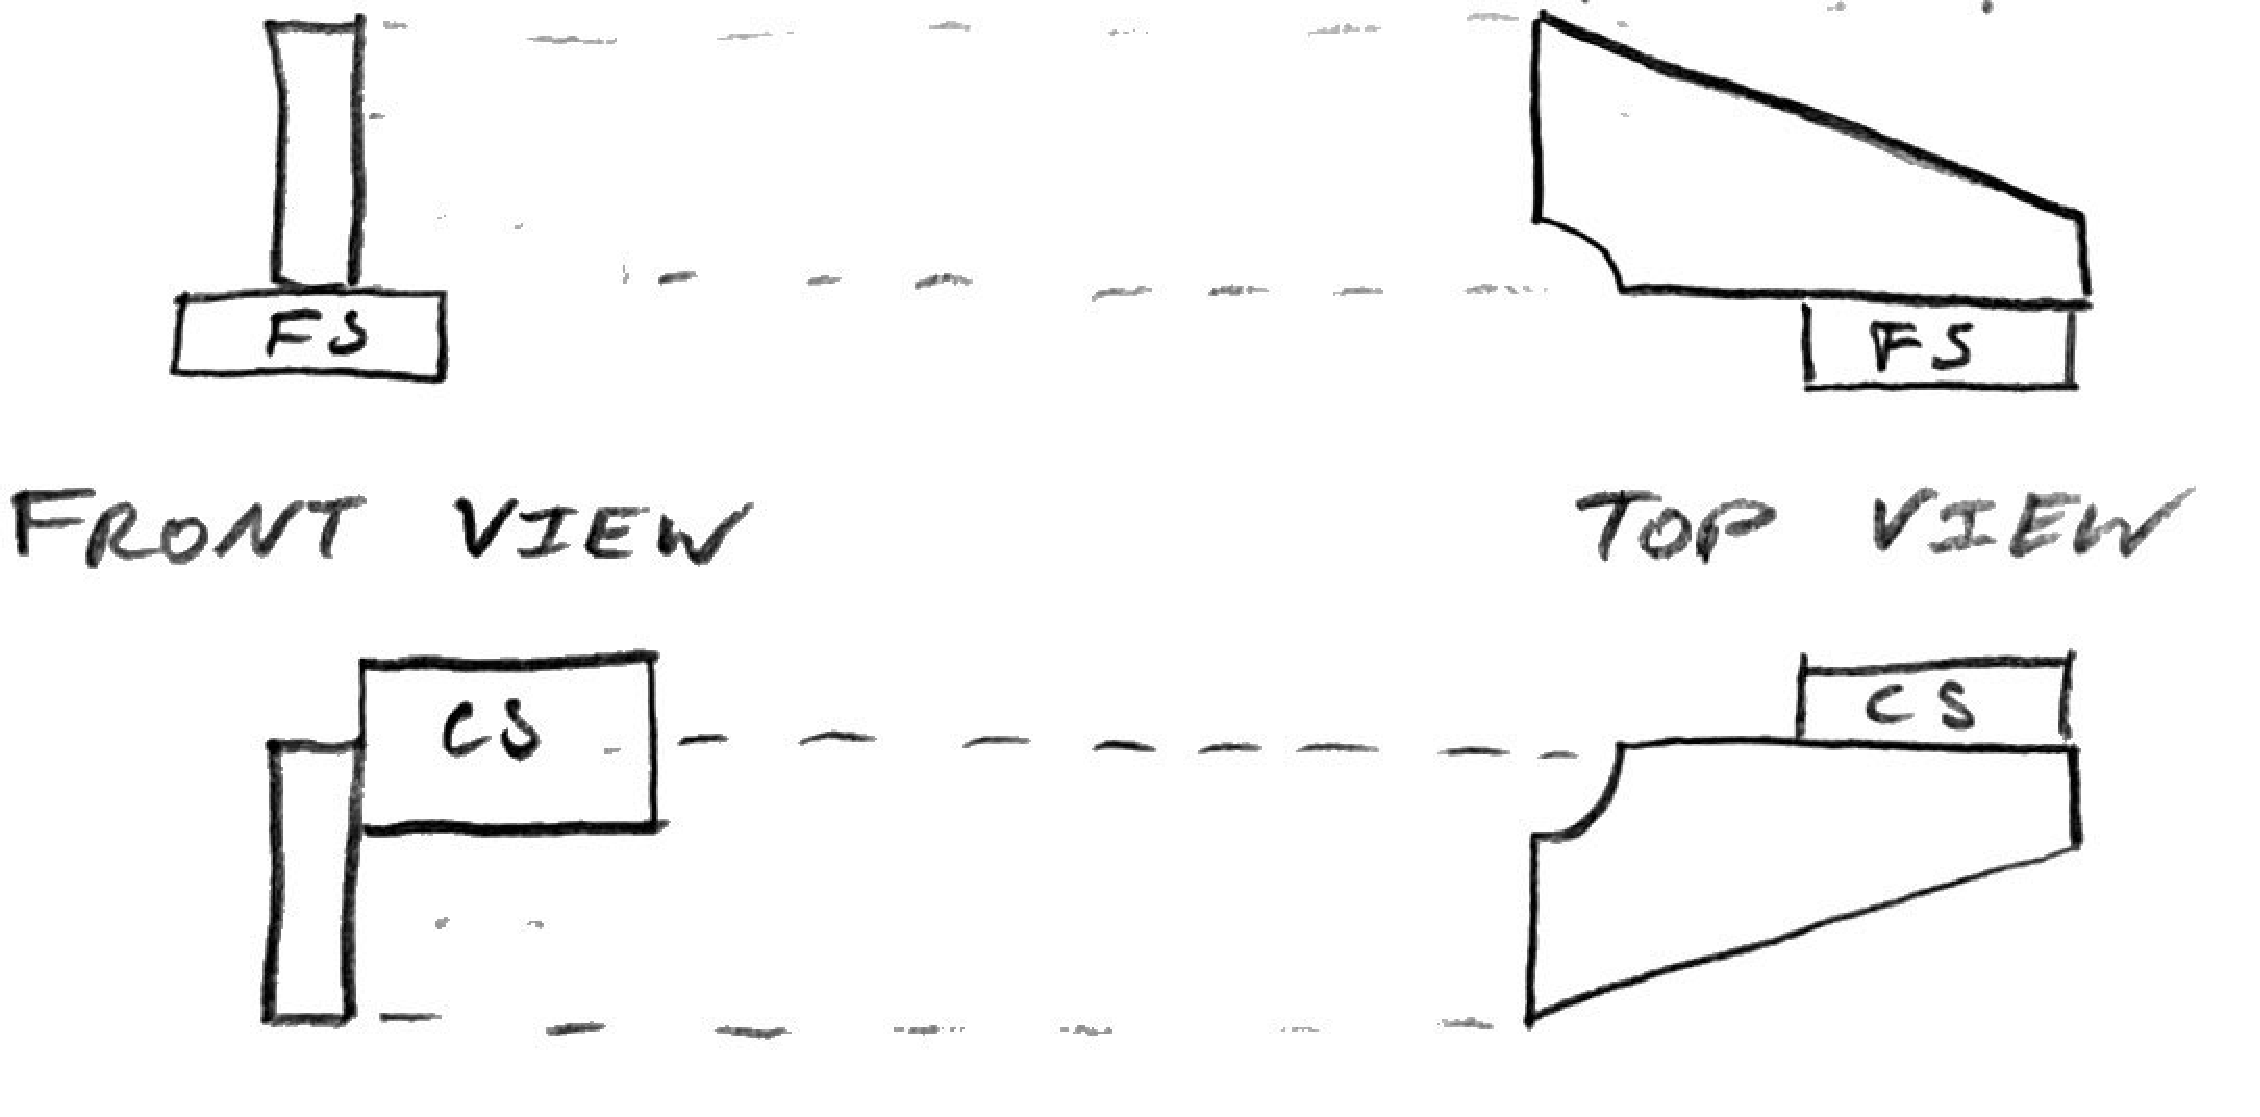
\includegraphics[width=0.5\linewidth]{Images//Designs/Design3b.pdf}
    \caption{Design 3b --- Box property detection platform with IRS}
    \label{fig:design3b}
\end{figure}
\begin{description}
    \item[Box Property Detection --]This iteration removes the property detection platform entirely and includes all relevant sensors on the gripper itself via 3D printed mounts. The color sensor will be mounted on one mandible, while a force-sensor, denoted \gls{FS}, using a timing-based algorithm to determine box size will be placed on the other.
\end{description}

\newpage
\section{Design 4}\label{sec:design4}
\begin{figure}[H]
    \centering
    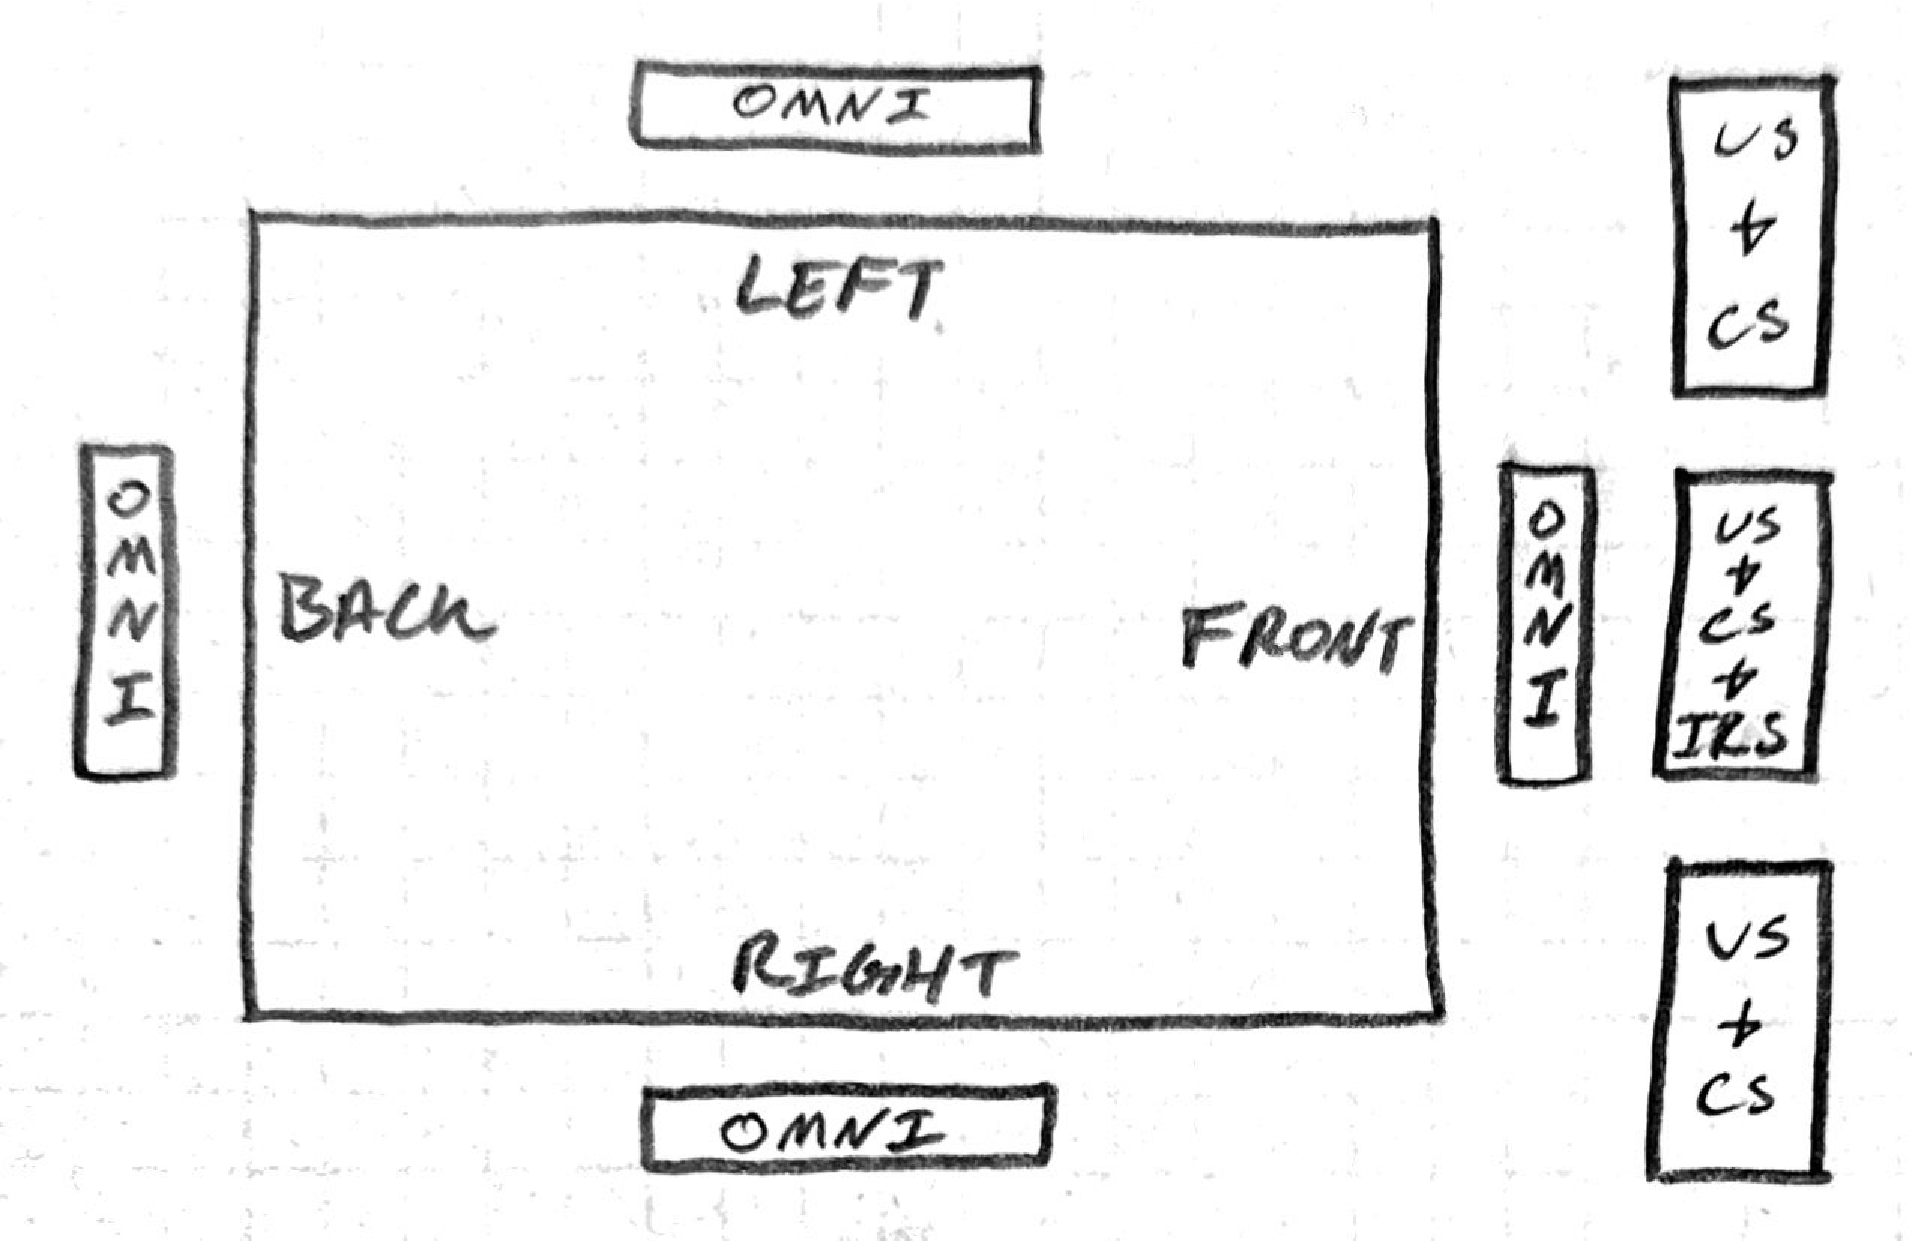
\includegraphics[width=0.5\linewidth]{Images//Designs/Design4a.pdf}
    \caption{Design 4a --- simplified layout of movement and sensor systems}
    \label{fig:design4a}
\end{figure}
The fourth design reorients the wheels as to be square against the sides, and combines the ideas for centralized sensors of \cref{sec:design2} and \cref{sec:design3}. This was chosen as the final design; the decision matrix supporting this design ca
\begin{description}
    \item[Wheel Configuration --]The \glspl{omni} are now placed in a squared configuration to increase the maximum speed potential, as the cornered configuration has inherent losses in the cardinal directions --- those most relevant to the tasks presented.
    \item[Sensor Configuration --]This iteration uses the middle color sensor idea from \cref{sec:design2}, and the centralized \gls{IR} array and ultrasonic sensor from \cref{sec:design3}. Together, these sensors provide as much information about the robot's location and orientation as possible.
\end{description}
\begin{figure}[H]
    \centering
    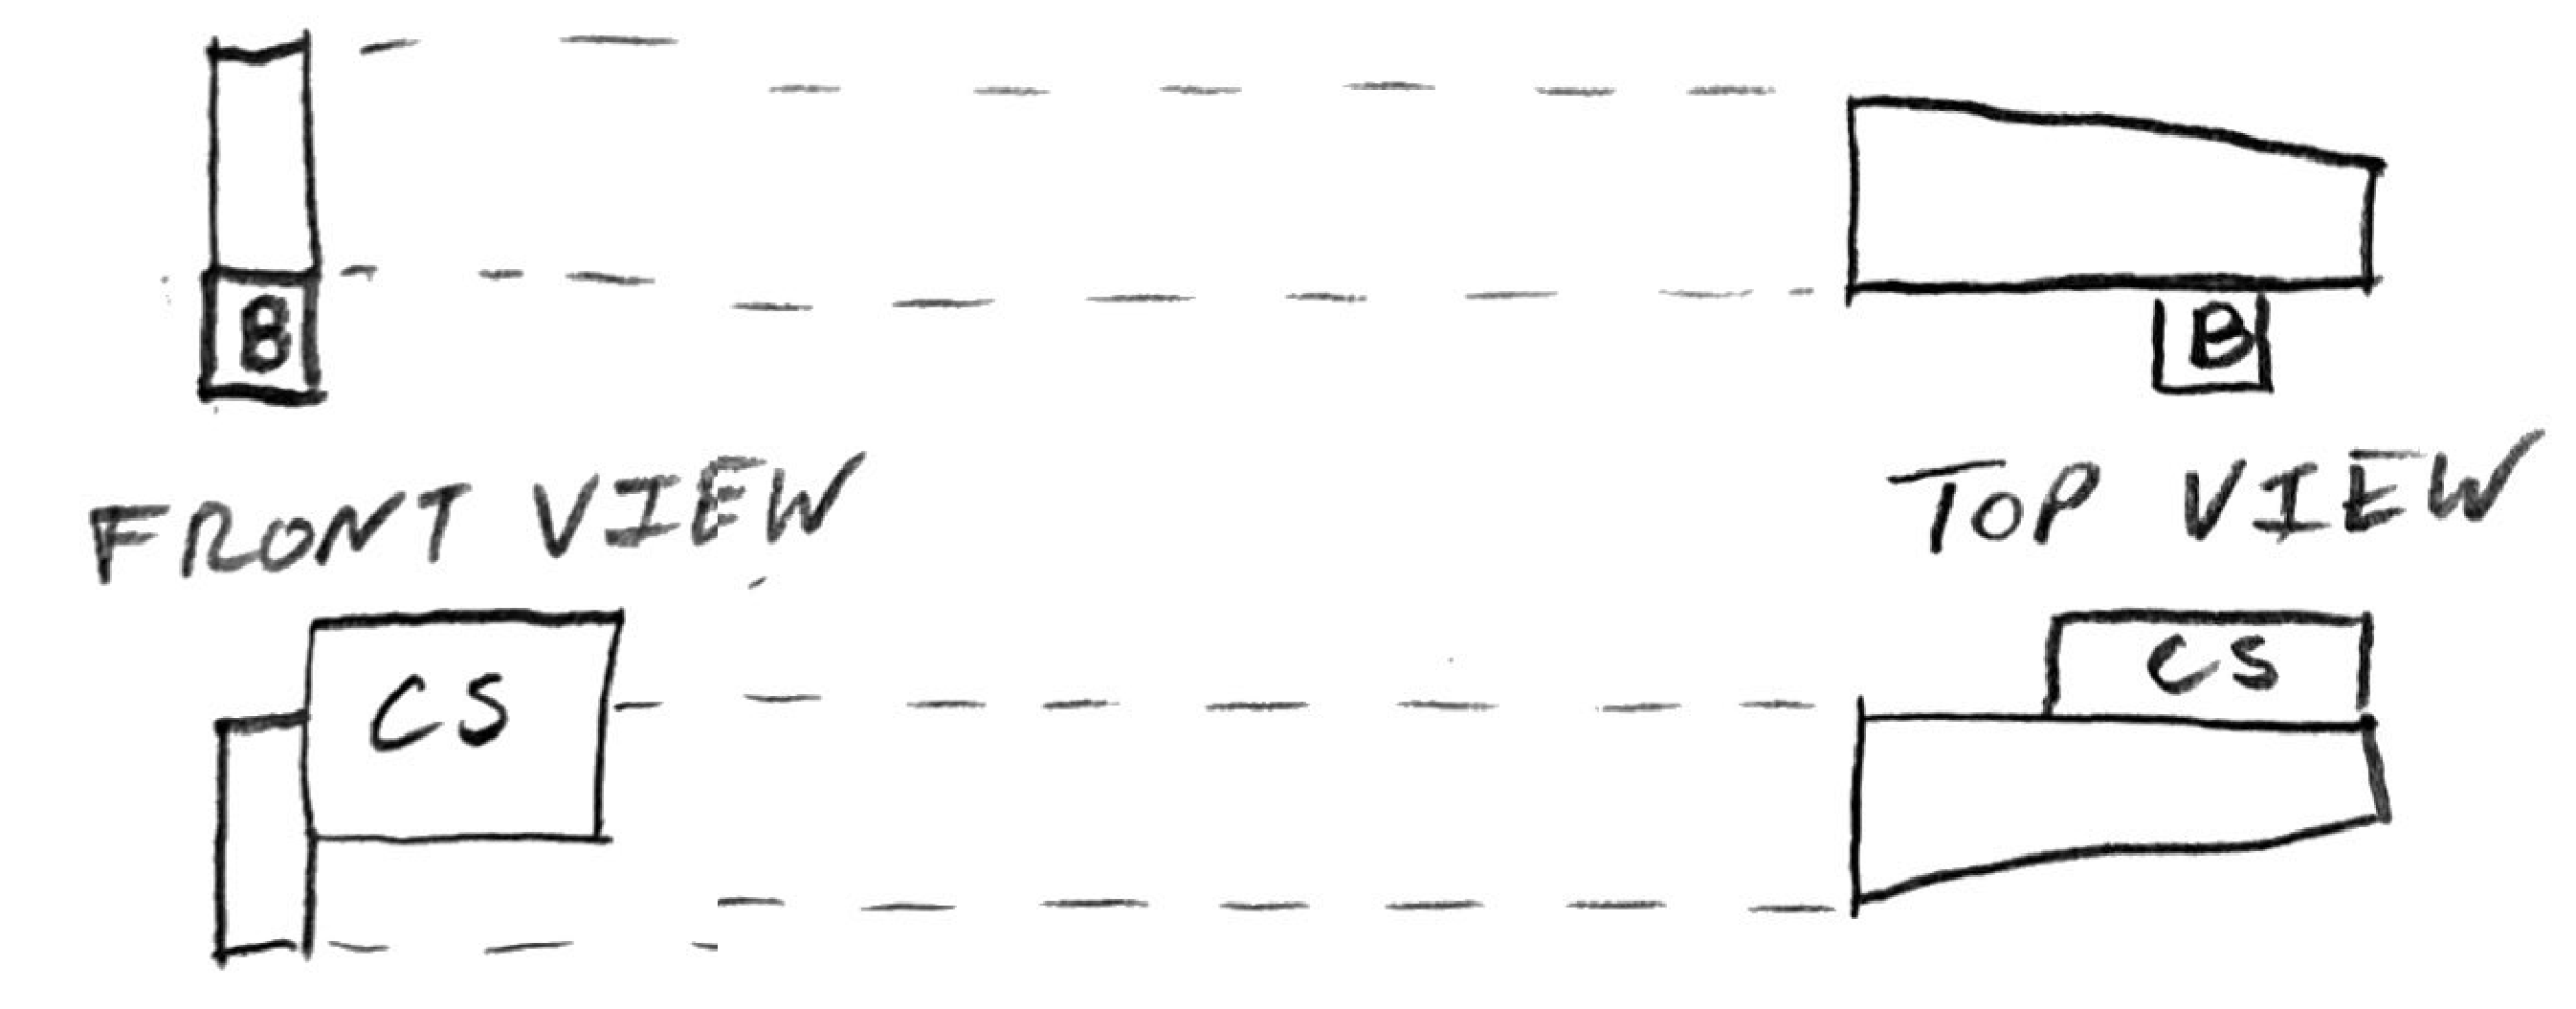
\includegraphics[width=0.5\linewidth]{Images//Designs/Design4b.pdf}
    \caption{Design 4b --- Box property detection platform with IRS}
    \label{fig:design4b}
\end{figure}
\begin{description}
    \item[Box Property Detection --]This gripper sensor layout is identical to the last with a button, denoted \gls{B}, in place of the force sensor, which will operate under a similar algorithm while eliminating the inconsistency of the force sensor.
\end{description}

\newpage
\section{Feasibility Analysis}\label{DecisionMatrix}
In order to compare these designs against one another, one must first create measures by which to rate each design, as well as decide how important each measure is to a theoretical successful project. The following measures, scored on a scale from 1-5, and their relative weightings were combined into a comparative table to create what is considered a decision matrix (\cref{tab:matrix}):
\begin{adjustwidth}{0.5cm}{0cm}
\vspace{1em}
\begin{description}
    \item[Programmability (1) --]Theoretical ease of programming when considering the number of sensors used and wheel configuration. This is weighted neutrally as the difficulty of creation should be considered negligible, but having the ability to edit the code as need be is crucial to problem solving.\vspace{1em}
    \item[Dynamicism (1.25) --]Theoretical ability to adapt to numerous circumstances, and how precise the resulting response should be to the ideal response. This is weighted moderately high as one of the design requirements is that the vehicle is adaptable, and increased dynamicism allows for more efficient objective completion.\vspace{1em}
    \item[Reliability (1.5) --]Ability to complete tasks repeatedly with minimal complications. Ideally, this system should perform 100\% of the time within the specified conditions; hence, this was weighted most severely.\vspace{1em}
    \item[Mechanical (-0.5) --]Presumed complexity of the mechanical system. It is weighted moderately negative due to the fact that repairs and modifications are harder on more complex systems, and it was crucial that potential mechanical issues are minimized because of the time constraint of this project.\vspace{1em}
    \item[Algorithmic Complexity (-0.25) --]Presumed complexity of the algorithm required for peak performance. This is weighted negatively in order to reduce the need for troubleshooting during creation, but less than that of Mechanical Complexity because a more complex algorithm could potentially increase performance.
\end{description}
\end{adjustwidth}

\begin{table}[h]
\centering
\begin{tabular}{|c|c|c|c|c|c|}
\hline
\multirow{2}{*}{\textbf{Metric}} & \multirow{2}{*}{\textbf{Weight}} & \multicolumn{4}{c|}{\textbf{Design}} \\ \cline{3-6}
 &  & \textbf{1} & \textbf{2} & \textbf{3} & \textbf{4} \\ \hline
Programmability  & 1      & 5       & 5       & 2       & 4       \\ \hline
Dynamism         & 1.25   & 1       & 2       & 3       & 5       \\ \hline
Reliability       & 1.5    & 1       & 2       & 4       & 5       \\ \hline
Mechanical Complexity & -0.5   & 0       & 0       & 5       & 3       \\ \hline
Algorithmic Complexity & -0.25  & 5       & 4       & 1       & 0       \\ \hline \hline
\multirow{2}{*}{\textbf{Score}} &     Weighted   & 12       & 13      & 15    & 17      \\ \cline{2-6}
&    Unweighted    & 6.5    & 9.5   & 9    & 16.25      \\ \hline
\end{tabular}
\caption{Comparison of design concepts via Decision Matrix}
\label{tab:matrix}
\end{table}

\newpage

\section{Design 1 (weighted total: 6.5)}\label{matrixdesign1}
\begin{greylineformat}
\begin{description}
    \item[Programmability (5) --]Given the extent of the team's experience with this base model, as well as the relative simplicity of design, coding the robot and debugging the code would be straight-forward.
    \item[Dynamicism (1) --]This iteration is incredibly outperformed by the others due to the small number of sensors and low-mobility wheel configuration. The sensor configuration simply does not provide enough information for the vehicle to perform acceptably.
    \item[Reliability (1) --]Again, the lack of fine-vehicle-control and data about the environment creates many reliability issues.
    \item[Mechanical Complexity (0) --]There is exactly enough on the vehicle to make it run well enough for learning/introductory purposes, but nothing more.
    \item[Algorithmic Complexity (5) --]Since there are no added features to assist in optimization, such as more sensors or increased mobility, creating an algorithm to complete the moderately complex tasks required of the robot would be a challenge. The only exception being the platform system, which would be easy to code and calibrate, but would also operate slowly when compared to other mechanisms.
\end{description}
\end{greylineformat}

\section{Design 2 (weighted total: 9.5)}\label{matrixdesign2}
\begin{greylineformat}
\begin{description}
    \item[Programmability (5) --]This configuration is now more mobile than the last with the addition of \glspl{omni} and there is an added color sensor centered between the existing ones, so not much has changed from a coding perspective. Additionally for the gripper platform, an ultrasonic sensor is easier to tune than an \gls{IR} sensor.
    \item[Dynamicism (2) --] The \glspl{omni} allow the vehicle to pivot which opens a lot of doors for movement, but the sensor configuration is still lacking.
    \item[Reliability (2) --] The added information from the new sensor means the vehicle can have less generalized, or more unique functions, which will aid significantly in preventing complications. Additionally, the outwardly-cocked ultrasonic sensors will detect objectives sooner than parallel sensors would.
    \item[Mechanical Complexity (0) --]Despite an added \glsxtrlong{DoF}, this vehicle is mechanically similar to the previous. 
    \item[Algorithmic Complexity (4) --]This iteration is only slightly better than the last with the added mobility and sensor making algorithms cleaner and more efficient.
\end{description}
\end{greylineformat}

\section{Design 3 (weighted total: 9)}\label{matrixdesign3}
\begin{greylineformat}
\begin{description}
    \item[Programmability (2) --]Swapping the middle color sensor for an \gls{IR} sensor array and adding a middle ultrasonic sensor adds a fair amount of complexity in the system when it comes to having multiple sensors interact. The new configuration of \glspl{omni} also creates an unintuitive movement system with a large potential for imbalances that are hard to debug.
    \item[Dynamicism (3) --]The new \gls{omni} configuration does, however, allow both crab-walking and cardinal translation, increasing overall efficiency of the wheels.
    \item[Reliability (4) --]The vehicle base and associated sensors are still about as reliable, if not more, than the previous, but the new gripper mechanism utilizes a force sensor which has been notoriously unreliable and difficult to calibrate.
    \item[Mechanical Complexity (5) --]The wheel configuration and use of a force sensor make this system overly complex.
    \item[Algorithmic Complexity (1) --]Ignoring the individual difficulties of components, this vehicle has the potential for high performance without too many complicated unique functions given its mobility.
\end{description}
\end{greylineformat}

\section{Design 4 (weighted total: 16.25)}\label{matrixdesign4}
\begin{greylineformat}
\begin{description}
    \item[Programmability (4) --]At this point, there are more sensors than are necessary, so there is a high degree of optimizations and redundancies that can be put in place to get around complications. Additionally, this allows for future modifications of the algorithm without the need to change the robot itself in any way.
    \item[Dynamicism (5) --]The movement system has been corrected to be relatively square to make fixing motor-imbalances easier, and make the movement system more intuitive for the user for easier troubleshooting.
    \item[Reliability (5) --]The button functions superior to the force sensor because the button requires more force than is necessary to hold the box while successfully avoiding damage.
    \item[Mechanical Complexity (3) --]This design is moderately complex both mechanically and electrically, as such, there are a great number of components on a fairly compact frame. This makes modifications and repairs incredibly difficult without sufficient care taken for wire/component management.
    \item[Algorithmic Complexity (0) --]Unique algorithms can be written for each step towards an objective, or remedy any of the complications along the way due to the vast sensors at the robot's disposal, making the overall algorithm relatively simple.
\end{description}
\end{greylineformat}
\end{document}